% Manuscript for Computers & Security (Elsevier). Build: latexmk -pdf main.tex
% Revision 7, after the seventh Reviewer 2 report. Every number comes from
% ../results/evaluation.json, ../results/counter_study.json, ../results/round5_analyses.json, ../results/condition_check.json
% or ../results/performance*.json (results at release 2.9.0; the 2.8.0 results are in ../results/historical_2.8/); ../results/headline_numbers.md maps headline figures to their JSON paths.
\documentclass[preprint,12pt]{elsarticle}

\usepackage{amsmath}
\usepackage{booktabs}
\usepackage{graphicx}
\usepackage{float}
\usepackage{array}
\usepackage{xurl}
\usepackage[hidelinks]{hyperref}
\usepackage{lineno}
\graphicspath{{figures/}}
\makeatletter\newcommand{\tablerows}[1]{\@@input #1 }\makeatother % generated rows: scripts/paper_tables.py
\renewcommand{\topfraction}{0.95}
\renewcommand{\textfraction}{0.05}
\renewcommand{\floatpagefraction}{0.8}
\setcounter{topnumber}{3}
\setlength{\emergencystretch}{2em}

\journal{Computers \& Security}

\begin{document}

\begin{frontmatter}

\title{Counting Versus Testing the Destination: A Simulation Study of Layered Defences Against SMS OTP Flooding and Pumping}

\author[inst1]{Naveed Ahmed\corref{cor1}}
\ead{optimistbs@gmail.com}
\cortext[cor1]{Corresponding author.}
\affiliation[inst1]{organization={Affiliation to be completed before submission},
            country={Saudi Arabia}}

\begin{abstract}
Endpoints that send one-time passwords by SMS are abused to waste money (flooding) or to earn part of the termination fee (SMS pumping). We evaluate in simulation a twelve-step defence that draws trust from app attestation, signed sessions and verification outcomes, against simpler designs and 25 attacker profiles. Attacks with a signature in the request are contained at little cost to simulated users; a residential attacker with farmed CAPTCHA scores is rationed by refusing half of first-time users. On the destination, short-window counters of SMS sends per number block, selected at a benign service target, leaked 6 to 48 messages against four concentrated 20-minute pumpers at 0.06 to 0.43 points of attack-free completion, where at the busiest density the default sequential tests of verification outcomes leaked 19 to 452. Under a second predeclared protocol on unseen seeds and workloads, the frozen counter met its leakage and benign-cost claims, leaked no more than the tests in all but 13 of 144 cells, all against an instantly verifying carrier, and failed both service-under-attack claims when the pumper shares blocks with real users. For attacks of up to an hour, unfitted estimates ordered the two policies' mean leakage in all 18 decisive boundary cells: the counter loses its advantage against paced or widely spread pumpers.
\end{abstract}

\begin{keyword}
SMS pumping \sep artificially inflated traffic \sep one-time password \sep rate limiting \sep sequential tests \sep fraud prevention
\end{keyword}

\end{frontmatter}

\linenumbers

% ---------------------------------------------------------------------------
\section{Introduction}
\label{sec:intro}

Most online services verify a phone number by sending it a code by SMS, from an endpoint reachable before any account exists, at a tenth of a cent to twenty cents a message. A flooder makes the service send to numbers it does not own; a pumper sends to a range whose operator shares the termination fee, turning the service's SMS budget into its income~\cite{mitre_t1496_003}. Twitter's owner said in 2023 that pumping had cost the company about 60 million dollars a year~\cite{commsrisk2023twitter}, and Huh et al.\ found as many attack requests as genuine ones in three months of one large service's logs~\cite{huh2025ait}.

This paper starts from such an incident on a registration flow the author operated, and from the redesign that followed: a twelve-step pipeline with attested platforms, signed sessions, number checks before a message is paid for, reputation from whether codes were entered, a five-response risk score and a hard budget. We ask in simulation which attacks it contains against simpler designs, at what cost in completed registrations (RQ1); which layer is responsible (RQ2); when outcome-based reputation separates an attacker from simulated users (RQ3); what rationing costs when it does not (RQ4); and what destination policies cost legitimate users, with and without an attack (RQ5).

The destination became the centre of the study, because a pumper is paid only on its partner's ranges: under a predeclared comparison a plain counter of sends per number block leaked less than our sequential tests of code outcomes, and a second predeclared protocol mapped where that holds and fails. We contribute eight gaps identified through recollection and subsequent design review, as motivation only, the design and an open implementation, measurements of where reputation stops separating and what rationing depends on, both destination-policy comparisons with their failures and collateral damage, and unfitted estimates of when counting leaks less than our tests; Sections 7.1--7.4 are context for the destination results (Sections 7.5--7.7).

% ---------------------------------------------------------------------------
\section{Background and related work}
\label{sec:related}

\paragraph{Revenue-share fraud}
In international revenue share fraud, traffic is generated to an advertised number range and the termination fee is split along the route~\cite{sahin2017sok}. Sahin and Francillon's 3.14 million test numbers from twelve providers show the range to be the fraudster's managed asset~\cite{sahin2021irsf}.

\paragraph{Detecting artificially inflated SMS}
Huh et al.\ trained gradient-boosted trees on 9.4 million SMS authentication logs from nineteen countries, reaching 89.6\% recall at 0.19\% false positives on web traffic~\cite{huh2025ait}. About 73\% of web attacks sent four or fewer requests per identity a day, defeating per-entity limits, and destination signals were the strongest: about 92\% zero conversion for attacks against 21\% for genuine traffic. Their detector needs labelled traffic and acts per request on request, history and country features. Their data show that destination aggregation is informative; what we add is a controlled comparison of two label-free ways to act on it per block, from send counts or code outcomes, and of their cost to users who share a block. Theirs was not reproduced, so the two are not ranked.

\paragraph{Defences in practice}
Twilio's Fraud Guard blocks regions known for pumping~\cite{twilio_fraudguard}, and its SMS Pumping Risk Score advises friction from 60 and refusal above 90~\cite{twilio_pumping_risk}, so graded destination action is established practice; no product was benchmarked. CAPTCHA solving is a labour market at about a dollar per thousand~\cite{motoyama2010captcha}, open where machine solvers fail~\cite{dionysiou2020captcha}; client puzzles~\cite{dean2001puzzles} were not evaluated. Residential proxy addresses rotate within minutes~\cite{mi2019resip}, and carrier-grade NAT makes address reputation on cellular networks ``all but infeasible''~\cite{richter2016cgn}.

\paragraph{Identity and change detection}
One entity can present many identities~\cite{douceur2002sybil}; a signed session gives continuity, not scarcity. Our block tests are Wald's sequential tests~\cite{wald1945sprt} run as Page's cumulative sums~\cite{page1954cusum}. Quickest change detection minimises delay under false-alarm constraints~\cite{veeravalli2012qcd}, and a CUSUM's parameters follow from the error rates it must meet~\cite{nist_cusum}; windowed statistics and confidence sequences~\cite{howard2021confseq} were not evaluated, so `testing' below means our conversion and speed tests only. Step~7 resembles risk-based authentication~\cite{wiefling2019rba}; attacks on the code once sent are a separate problem~\cite{mulliner2013smsotp,siadati2017sms}.

% ---------------------------------------------------------------------------
\section{The incident and the adapted attacker}
\label{sec:incident}

This section is motivation, not evidence: no logs from the period are in our hands, permission to describe it is pending, and no result depends on it. The flow sent an SMS to any unregistered number. The first controls, v1, were reCAPTCHA v3 on web requests, one message per number per minute, five requests per address per minute, a country allow-list, a body-length limit, a proxy block and per-platform caps. The returning abuse used thousands of residential addresses, carried the iOS header to skip the CAPTCHA, and stayed under every limit.

\begin{table}[H]
\caption{The v1 controls and their gaps, recalled by the operator from the incident (Recalled; not supported by logs) or found in the design review that followed (Review).}
\label{tab:v1}
\footnotesize
\begin{tabular}{clp{4.6cm}p{5.0cm}}
\toprule
Gap & Source & v1 assumed & How it fails \\
\midrule
A & Recalled & A platform header says which app sent the request & Sending the header reached every exemption \\
B & Recalled & Five requests per address per minute bound an attacker & A fresh residential address per request \\
C & Recalled & A number given is worth sending to & Generated numbers cost as much as real ones \\
D & Review & An allowed country is a safe destination & Premium ranges inside it cost far more \\
E & Recalled & Per-key caps bound total spend & A wide attack under every cap \\
F & Review & Check-then-increment is a rate limit & Two racing instances both pass \\
G & Review & Bulk and test flags are internal & Neither needs stronger authentication \\
H & Review & Each check says which check failed & Thresholds can be probed one at a time \\
\bottomrule
\end{tabular}
\end{table}

\paragraph{Threat model}
\label{sec:threat}
The attacker wants as many messages sent as possible, or sent to numbers that pay it. It buys residential proxies and human-like reCAPTCHA tokens (about 0.3 cents each), mints fingerprints, generates numbers and knows the thresholds. A pumper also has a colluding operator's ranges, where it may enter codes, report deliveries as failed, build verified history, spread over blocks and buy challenge solutions. It cannot forge an attestation, use ranges its partner does not terminate, or make a stranger enter a code.

% ---------------------------------------------------------------------------
\section{Design}
\label{sec:design}

No message is paid for before every check passes, and cheap checks run first. Trust comes from evidence the client cannot forge, an attestation, a server-signed session and the fate of earlier codes, though such evidence can be manufactured (Section~\ref{sec:adaptive}).

\subsection{The pipeline and the risk score}

A request passes the steps of Table~\ref{tab:steps} until one refuses it. Step~0 takes the platform only from a valid App Attest or Play Integrity result. Each limit and reservation is one atomic Redis operation, but the enclosing steps are not one transaction: on the normal path a refused request gives back its per-number claims and counter slot, and the hourly budget is reserved only for a message about to be enqueued, a reservation rather than a completed dispatch; a crash between them can leak reservations (Section~\ref{sec:method}). Address limits and source caps count requests, except that a request Step~11 challenges gives its source-cap count back. Every outcome after Step~0 except the challenge returns one HTTP~200 body after at least 400\,ms, a floor that cannot hide longer work.

\begin{table}[H]
\caption{The twelve steps (the v1 gaps of Table~\ref{tab:v1} they address in brackets). FB is the feedback loop.}
\label{tab:steps}
\footnotesize
\begin{tabular}{cp{11.6cm}}
\toprule
Step & Check \\
\midrule
0 & Proxy block; platform from attestation, never from the header [A] \\
1 & Signed session bound to a fingerprint; 3 requests per session per 10 min [B] \\
2 & Limits per address, /24 and ASN, lower for hosting ASNs [B, F] \\
3--4 & reCAPTCHA v3 threshold and origin check, web only \\
5 & Number intelligence: cost class, sequential numbers, liveness; reads the block's verdict stage [C, D, G] \\
6 & Body length, excluded numbers; test bypass needs a credential [G] \\
7 & Risk score and tier: allow, delay, challenge, downgrade, block [H] \\
8 & Per-number backoff, 60\,s doubling to 1\,h, five a day \\
9 & Per-source, platform and country caps with an adaptive multiplier \\
10 & Operating mode: elevated above 80\% of the hourly budget, emergency at 100\% [E] \\
11 & Reserve hourly count, spend and any destination slot; write state; enqueue; uniform response [E, H] \\
FB & Outcomes per key; destination-block tests; denylist of fine keys \\
\bottomrule
\end{tabular}
\end{table}

Step~7 computes
\begin{equation}
s = \sum_i w_i x_i + w_c\,\frac{\max(0,\theta - r_{\min})}{\theta} + w_s\,f + w_m\,i - w_v\,v_n - w_f\,v_f,
\label{eq:score}
\end{equation}
where the $x_i$ are request signals (CAPTCHA score, hosting ASN, fingerprint age, session requests, country mismatch, number class), $r_{\min}$ is the lowest conversion ratio over the request's keys (address to destination block), $\theta=0.3$, $w_c=25$, $f$ and $i$ flag a flooded key and one whose codes are entered within seconds, and $v_n$, $v_f$ mark a number and fingerprint with verified history; other weights are 5 to 25~\cite{otpguard2026}. Tiers start at 20, 40, 60 and 80: \emph{allow}; \emph{delay} (a doubling wait); \emph{challenge} (credits $-20$ when solved); \emph{downgrade} (push or WhatsApp, never SMS); \emph{block}. 

\subsection{The feedback loop}
\label{sec:feedback}

A send resolves as \emph{verified} when its code is entered, \emph{failed} after five wrong attempts or two minutes past the delivery receipt, and \emph{undelivered} without a receipt in sixty seconds or with a failure receipt; only the first two feed reputation. A positive receipt after a negative one reopens the send; a late verification reclassifies it, but an issued verdict stands. Each transition records its effects and its time in the same compare-and-set, and a recovery sweep finishes a dead process's work; each effect type applies at most once, and exactly once if the sweep runs within 20 minutes. Reputation counts land in the transition's hour and a block keeps its latest outage failure time, but a block's statistic accumulates in processing order and a verdict is dated at the event that completes the crossing, so a late event can backdate a verdict that contains later evidence, moving its expiry and the next test's start (by ten minutes in one diagnostic). Events arrive in time order on the live path and in every simulated run.

\subsection{Destination policies}
\label{sec:blocks}

A pumper is confined to its partner's ranges but can rotate numbers and blocks within them. Destination policies are keyed on the 8-digit block (10\,000 numbers), so their protection weakens as a pumper spreads.

\paragraph{Sequential tests}
The conversion statistic assumes users verify with $p_\ell = 0.8$ and a flooder with $p_a = 0.1$: a failure adds $\ln\frac{1-p_a}{1-p_\ell} = 1.50$, a verification $\ln\frac{p_a}{p_\ell} = -2.08$. The speed statistic assumes a machine enters a verified code within five seconds with $q_a = 0.9$ and a person with $q_\ell = 0.2$, since autofill removes the keystroke~\cite{google_smsretriever,wicg_webotp}; it adds $1.50$ or $-2.08$. A verdict is issued, and the statistic reset, when either exceeds $h = \ln 1000 = 6.91$. The floor $S_t = \max(-ch,\, S_{t-1} + \text{increment})$ sets the memory: unbounded $c$ is Wald's test, $c = 0$ Page's cumulative sum; the default is $c = 1$. A first verdict makes the block's first-time clients pass a challenge for an hour; a second within the hour moves them off SMS, refusing those without another channel.

\paragraph{Counters}
A counter limits SMS sends per block in a daily or short refilling window. Step~11 reserves a slot and decides the stage in one atomic operation when an SMS is about to go out, so concurrent requests cannot skip the challenge. Past the limit a graded counter challenges first-time clients, and past twice the limit moves them off SMS; a refusing counter refuses. Clients with verified history are exempt from both policies, so a code entered on a pumper's number can buy that number an exemption. A token bucket of the same rate (burst 4 or 12; its challenge-tier bucket refills independently, whereas RFC~2697's excess bucket fills only from the committed one~\cite{rfc2697}) and the counter combined with the tests were explored as alternatives.

\subsection{Capacity controls}

Step~9 multiplies its caps by 0.25 to 1.5 according to a baseline job comparing each key with its expected rate, learned from the pipeline's hourly counters; without history the static cap stands. Verified history avoids the adaptive reduction, not the static caps or the budget, which bounds SMS count and spend, not vendor or fallback costs.

% ---------------------------------------------------------------------------
\section{Leakage estimates and a heuristic crossover}
\label{sec:model}

We compare the SMS sent to a pumper's numbers over an attack of $T \le 60$ minutes, by a pumper that solves no challenge and holds no verified history. Against the sequential tests, one reaching $B$ blocks with $N$ requests at rate $\lambda$ leaks about
\begin{equation}
L \approx \min\bigl(N,\; kB + \lambda\,\tau\bigr), \qquad k = \lceil h/1.50 \rceil = 5,
\label{eq:leak}
\end{equation}
before its first verdict, where $\tau$, the time a send stays unresolved, is the resolution timeout plus the delivery delay plus half the timeout worker's period (2.55 minutes) if the carrier never verifies, and seconds if it verifies at once. Judged, such a pumper is held for the verdict's hour, so for $T \le 60$ Equation~\eqref{eq:leak} also estimates the attack's total; it ignores prior credit and outage suspension. A carrier verifying a share $\sigma$ of codes with human-like delay gives the conversion statistic an expected increment of $\sigma(-2.08) + (1-\sigma)(1.50)$, zero at $\sigma^{*} = 0.42$; above it the statistic drifts away from a verdict.

A counter of $q$ sends per block opens a window with a block's first reserved SMS and closes it after the window length. A pumper that finds its blocks' counters empty (a cold start) sends at most
\begin{equation}
L_c \le \min\bigl(N,\; q B w\bigr), \qquad w = \lceil T / \text{window} \rceil,
\label{eq:counter}
\end{equation}
whatever its carrier does with the codes. If a legitimate send has already opened a window on block $b$, using $c_b \ge 1$ slots, the pumper can also take the remaining $(q-c_b)^+$ before at most $w$ further windows open, so in general
\begin{equation}
L_c \le \min\Bigl(N,\; q B w + \textstyle\sum_{b\ \mathrm{open}} (q - c_b)^+\Bigr) \le \min\bigl(N,\; B\,(q w + q - 1)\bigr).
\label{eq:counterwarm}
\end{equation}
Solving challenges doubles these bounds, and verified history exempts a client from them. While neither policy's estimate reaches $N$, the cold-start bound lies below the tests' estimate when
\begin{equation}
B\,(q w - k) < \lambda\tau,
\label{eq:cross}
\end{equation}
and a warm start adds the residual quota to the left side. Equation~\eqref{eq:cross} is the algebraic crossing of two simplified quantities, neither an empirically established switching point nor a necessary condition: other limits can hold either policy below its estimate. A carrier that games outcomes may never be judged, so the tests' leakage approaches $N$.

In the code every send takes a slot, verified clients' included. If a block's sends arrive as a Poisson stream with mean $m$ per window and all reach the counter, a window holds $1 + X$ of them, $X \sim \mathrm{Poisson}(m)$, and the idealized share beyond the quota is $E[(1+X-q)^+]/(1+m)$: 7.3\% at $m = q/2$ and 27\% at $m = q$ for $q = 4$. It is not a challenge rate: exempt clients take slots without challenge, and challenge failures, the second tier and earlier gates are ignored. Equations~\eqref{eq:counter}--\eqref{eq:cross} and $k$ follow from the rules, $\tau$ from the configuration and $\lambda$ from the attack; what an excess send costs a user needs the simulation.

% ---------------------------------------------------------------------------
\section{Implementation and evaluation method}
\label{sec:method}

\paragraph{Implementation}
About 4\,000 lines of Python implement the pipeline, feedback loop and vendor adapters on in-memory and Redis backends. Up to release 2.8.3 the simulator's in-memory store let a sorted set expire a fixed time after its first write, whereas Redis keeps it while it is written to, so in simulation the outage detector and Step~5 lost recent observations. Release 2.9.0 makes the in-memory store keep state as Redis does, which differential tests check operation by operation and on whole simulations, and every study was rerun with it. Earlier releases repaired seven replay and concurrency defects, each with a regression test. Of 453 tests, 19 use a real \texttt{redis-server}, eighteen of them testing specific interleavings of two instances, not all. Step~11 is still not one transaction: a crash after its reservations leaks reserved slots or resolves the send as undelivered. The implementation is a research prototype.

\paragraph{Simulation}
\label{sec:sim}
The pipeline runs against scripted vendor fakes on a simulated clock. After a warm-up of ten minutes (30 or 130 for pumping), attacks run over legitimate traffic at 20 requests per minute. Simulated users verify 80\% of codes after a lognormal delay (median 22\,s; 2\,s for the 20\% using autofill); 70\% of numbers are reachable on WhatsApp; 90\% of users complete a challenge; 20\% are returning account holders with a stable fingerprint, a trusted number and verified history, so results for returning users describe trusted identities only. Separate random streams give all scenarios at a seed the same users.

Three behavioural parameters have published counterparts: genuine conversion (one provider's 68\% or more~\cite{twilio_verify}; ours 60 to 90\%) and the never-converting destinations and identity churn of Section~\ref{sec:related}, which our non-verifying pumpers and one-use farm share; the rest are assumptions. Attackers (Table~\ref{tab:attackers}) draw pool size, rate and CAPTCHA class per seed; in a nested design (ten configurations, three seeds each) these draws account for 92\% [80, 98] of the variance of the farm's leakage. Brackets are 95\% percentile-bootstrap intervals, paired per seed for differences; they describe variation under this generator, not uncertainty about real traffic.

\paragraph{Two protocols and their chronology}
Table~\ref{tab:studies} maps the studies. The first protocol, committed before its runs, fixed the matched comparison and a robustness study over twelve Latin-hypercube points (conversion 0.6--0.9 and five other behavioural parameters) and a held-out family (60 to 120 attack requests a minute, 50\,000 to 500\,000 addresses, heterogeneous legitimate traffic), with claims C1--C5 that hold if true in 90\% of cells, a benchmark convention, not a confidence level. The matched comparison changes only the destination policy and, at three block densities, selects on tuning seeds the least leakage summed over four concentrated pumpers among settings at or above the \emph{tuning target}, the default's completion minus 0.5 points (the full sequential grid only at the busiest). The robustness study's first run failed C1 in 32 of 108 cells because attack and no-attack runs drew different users; we fixed the pairing, a fix that followed a result, and reran every study. The second protocol (claims K1--K5) was written after the matched comparison had selected three counters and committed before its runs; six of its seed values had served other robustness points, never selection. Both were rerun unchanged with 2.9.0 (9\,919, 7\,925 and 240 runs, each carrying its code hash); against 2.8.0, total leakage changed in 855 of 17\,964 comparable runs, but no claim, eligibility or selection used here did (change report in the artifact).

\begin{table}[t]
\caption{The studies, their seeds (three per shifted point), attack durations and results. MC: Monte Carlo.}
\label{tab:studies}
\scriptsize
\begin{tabular}{@{}>{\raggedright\arraybackslash}p{4.2cm}>{\raggedright\arraybackslash}p{2.6cm}>{\raggedright\arraybackslash}p{1.9cm}>{\raggedright\arraybackslash}p{3.6cm}@{}}
\toprule
Study & Seeds & Attack & Results \\
\midrule
Designs; ablation, interactions & 0--29; 0--9 & 20 min & Table~\ref{tab:headline}; Section~\ref{sec:rq2} \\
Dilution; score and cap sweeps; cadence & 0--4; 0--9 & 60; 20 min & Sections~\ref{sec:separability}, \ref{sec:rationing} \\
Pumping and spread & 0--9 & 20 (60) min & Table~\ref{tab:pumping}; Section~\ref{sec:pumping} \\
False alarms; poisoner; adaptive attackers & MC; 0--4, 0--7, 0--9 & 24\,h; 20--70 min & Sections~\ref{sec:fp}, \ref{sec:adaptive} \\
Protocol 1: matched comparison & tuning 100--102; 0--9 & 20 min; 24\,h benign & Table~\ref{tab:matched}; Figures~\ref{fig:matched}, \ref{fig:matchedpaired} \\
Protocol 1: robustness, C1--C5 & 12 points & 20 min; 6\,h benign & Sections~7.1--7.7 \\
Protocol 2: E1 attacked service & 300--309 & 60 min & Table~\ref{tab:attacked} \\
\quad E2 held-out family, K1--K5 & 12 points & 20 min & Table~\ref{tab:claims} \\
\quad E3 adaptive; E4 boundary & 300--309; 300--304 & 20--360 min & Section~\ref{sec:matched}; Figure~\ref{fig:boundary} \\
\quad E5 selection, every density & tuning 100--102; 300--309 & 20 min; 24\,h benign & Section~\ref{sec:matched} \\
\bottomrule
\end{tabular}
\end{table}

\paragraph{Designs and metrics}
Seven designs: \textbf{v1} (header-trusted platform, static caps), \textbf{v1-corrected} (attested platform), \textbf{budget-only} (sessions, static caps, budget), \textbf{block-limit} (a refusing counter of five sends per block per day), \textbf{conversion-only} and \textbf{speed-only} (v2 minus one block test), and \textbf{v2}. A seed is \emph{contained} when leakage stays at most 5\% of the attack rate from some minute to the window's end, for at least five minutes. \emph{Attributable} loss compares the same requests with the policy enforced and absent, net of the reverse, in points of offered users: on attack-free traffic it is the \emph{benign cost}, on the attacked trace the \emph{extra harm} relative to the attacked no-policy arm. \emph{Degradation} compares the attacked trace with attack-free operation under the same policy.

\begin{table}[H]
\caption{The 25 attacker profiles by capability, and the destination policies each faced: S, sequential tests; C, counters; B, block-limit. Names and parameters: \texttt{results/\allowbreak attacker\_profiles.md}.}
\label{tab:attackers}
\scriptsize
\begin{tabular}{@{}>{\raggedright\arraybackslash}p{2.4cm}>{\raggedright\arraybackslash}p{9.4cm}l@{}}
\toprule
Capability & Profiles & Policies \\
\midrule
A signature in the request (5) & One address; datacenter rotation abroad; a premium-rate prefix; numbers walked upward; the farm with an unattested iOS header & S, B \\
Looks like a person (7) & Residential bot; farmed CAPTCHA with fresh or aged fingerprints; one 48-hour-old browser profile & S, B \\
 & Low and slow, 2 or 10 requests/min over 20 ASNs; datacenter rotation buying challenge solutions & S \\
Games outcomes or trust (8) & Pumpers on elevated-cost or standard ranges verifying within 1\,s, or 60\% after 30\,s & S \\
 & Threshold-aware and receipt-faking carriers; three trust builders (500 identity/number pairs verify for 10 or 30 min, then flood) & S, C \\
Concentrated on the destination (5) & Four pumpers on three blocks (carrier never verifies, verifies within 1\,s or 60\% after 30\,s, or buys challenges); a poisoner on users' blocks & S, C \\
Spread (generated) & 3 to 300 blocks, at full rate or at most the counter's quota per block & S, C \\
\bottomrule
\end{tabular}
\end{table}

% ---------------------------------------------------------------------------
\section{Results}
\label{sec:results}

\subsection{RQ1: what is contained, and at what cost}
\label{sec:rq1}

\begin{table}[t]
\caption{Leaked share (\%, mean of per-run shares) of about 600 attack requests in twenty minutes, thirty seeds, under v1, the block-limit design (BL) and v2 with source caps lifted, and under v2 with caps on, with the first-time users refused and all users completing (\%). All designs, with intervals: supplementary Table~S1 (\texttt{results/\allowbreak design\_table.md}).}
\label{tab:headline}
\footnotesize
\begin{tabular}{@{}lrrrrrr@{}}
\toprule
& \multicolumn{3}{c}{caps lifted: leaked} & \multicolumn{3}{c}{caps on, v2} \\
\cmidrule(lr){2-4}\cmidrule(lr){5-7}
Attacker & v1 & BL & v2 & leaked & refused & completed \\
\midrule
\tablerows{tables/headline.tex}
\bottomrule
\end{tabular}
\end{table}

Datacenter rotation leaks nothing under v2 because it scores in the challenge tier and declines challenges; Step~5 refuses the premium range, and the session cap holds the single client to two messages (Table~\ref{tab:headline}); in all 108 robustness cells these attacks leaked under 5\% at completion within two points of the paired no-attack run (claim C1). The walk leaks 61 [53, 70] messages before its block's verdict (block-limit: five), the reused profile 89 [83, 95].


The farm leaks 99.5\% with caps lifted under every design; v2's adaptive cap holds it to 229 [215, 244] messages, 46\%, by refusing 54\% [47, 60] of first-time users, so 45.5\% complete instead of 76.4\% under v1: rationing (claim C5 held in 36 of 36 cells).

\subsection{RQ2: conditional effects of each layer}
\label{sec:rq2}

In the ablation grid (90 effects, each conditional on all other layers, unadjusted intervals; artifact), removing the adaptive caps lets the farm leak 310 [194, 421] more messages; the risk engine, feedback loop and block key hold the walk by 166, 152 and 121 messages, and the loop holds the reused profile by 138. The key acts only through the loop (interaction $-121$ [$-141$, $-101$]).

\subsection{RQ3: where reputation stops separating}
\label{sec:separability}

A farmed-CAPTCHA attacker uses an address and fingerprint once and shares its country, prefix and residential ASN with every legitimate user, so the penalty its failures earn lands on everyone: over an hour with caps lifted (five seeds), up to twice the legitimate rate 99 to 100\% of it leaks: a shared key stays above 0.3 conversion until failures outnumber legitimate sends about 1.7 to one, and the conversion penalty alone reaches only \emph{delay}. At ten times, 70\% leaks while 17\% of legitimate users are challenged and 3.2\% refused (claim C2, at least 90\% leaked with caps lifted, held in 34 of 36 cells). Changing the risk score one setting at a time separates no better: a fresh-fingerprint weight of 40 stops the attacker only by challenging 47\% of legitimate users and refusing 8.5\%. In the settings run, reputation separated an attacker only on keys its sends dominated~\cite{douceur2002sybil}.

\subsection{RQ4: what rationing costs, and what it depends on}
\label{sec:rationing}

When separation fails, the cap is the lever: over ten seeds the default lets 47\% of the farm's requests through and refuses 41\% of all legitimate users, the tightest setting 20\% and 64\%. Both assume an oracle job told the legitimate rate, run every minute; every five minutes or hourly, it lets 75 to 96\% through. Learning the rate from the pipeline's counters, the deployed job leaks 193 [161, 229] messages with a clean three-week profile, 340 [239, 441] more on a cold start, 106 [62, 151] more with a stale profile and 45 [10, 77] more with a poisoned one.




\subsection{Pumping against the sequential tests}
\label{sec:pumping}

\begin{table}[H]
\caption{Concentrated pumpers on three blocks, caps lifted, ten seeds: messages leaked of about 574 requests in twenty minutes; seeds contained; mean minutes to containment (contained seeds) and to the first verdict (seeds with one); codes entered.}
\label{tab:pumping}
\scriptsize
\setlength{\tabcolsep}{2.5pt}
\begin{tabular}{@{}lllllr@{}}
\toprule
Carrier, design & Leaked & Contained & Containment & First verdict & Codes \\
 & (msgs) & (seeds) & (min) & (min) & entered \\
\midrule
\tablerows{tables/pumping.tex}
\bottomrule
\end{tabular}
\end{table}

In Table~\ref{tab:pumping} the speed test catches a carrier verifying within a second at 19 messages, while the carrier verifying 60\% with human-like delay is never contained: its first verdict comes at minute 11.6 on average and 452 messages leak (1\,067 in an hour). Claim C3 (containment with at most 30\% leaked) held in 36 of 36 cells.

Across 18 spread configurations leakage follows the blocks touched: with 30 blocks five to seven runs in ten are still contained. In the ten unsaturated configurations Equation~\eqref{eq:leak} errs by 1.6 to 7.9 messages per run (1 to 13\%); saturated, it overstates by up to 91.

\subsection{Destination policies: where the counter wins, and where it fails}
\label{sec:matched}

\begin{table}[H]
\caption{Matched comparison, first protocol, 200 blocks (144 legitimate sends per block a day), tuning seeds 100--102, evaluation seeds 0--9: twenty-minute leakage (messages) by never-verifying (NV), instant (IV), human-like (HL) and challenge-buying (CB) carriers; from 24-hour attack-free runs at 65\% conversion, completion, benign cost (points), users challenged and verdict events a day. Tuning target: 63.95\%.}
\label{tab:matched}
\scriptsize
\setlength{\tabcolsep}{3pt}
\begin{tabular}{@{}lrrrrrrrr@{}}
\toprule
Setting (selected as) & NV & IV & HL & CB & Compl. & Benign & Chall. & Events \\
\midrule
\tablerows{tables/matched.tex}
\bottomrule
\end{tabular}
\end{table}

\paragraph{At a benign service target}
Under the first protocol (Table~\ref{tab:matched}, Figures~\ref{fig:matched} and~\ref{fig:matchedpaired}), the sequential setting selected at the tuning target holds the human-like carrier to 126 messages only by raising 334 false verdict events a day, and falls 0.18 points below the target on seeds 0--9. The graded counter of four sends per block per ten minutes leaks 24 against each outcome-reading carrier and 48 against the challenge buyer, at 0.06 points; counters selected at the sparser settings leak 6 to 18 at 0.15 to 0.35 points (up to 0.43 at 80\%). With the full grid and density-specific attacks (E5) the rule selects the same counters, and so do other objectives on the tuning runs (worst-case leakage, a first-time-loss constraint, each attacker alone, 2\,000 random mixes), except the instant verifier alone and 3 mixes at 200 blocks; on fresh seeds the counter leaked least of the winners against every attacker but the instant verifier (25, against 15 and 16). On seeds 300--309 the 1\,000-block counter falls 0.12 points below its target, yet no seed-and-conversion cell fails the paired check (the evaluation default minus 0.5 points).

\begin{figure}[!tbp]
\centering
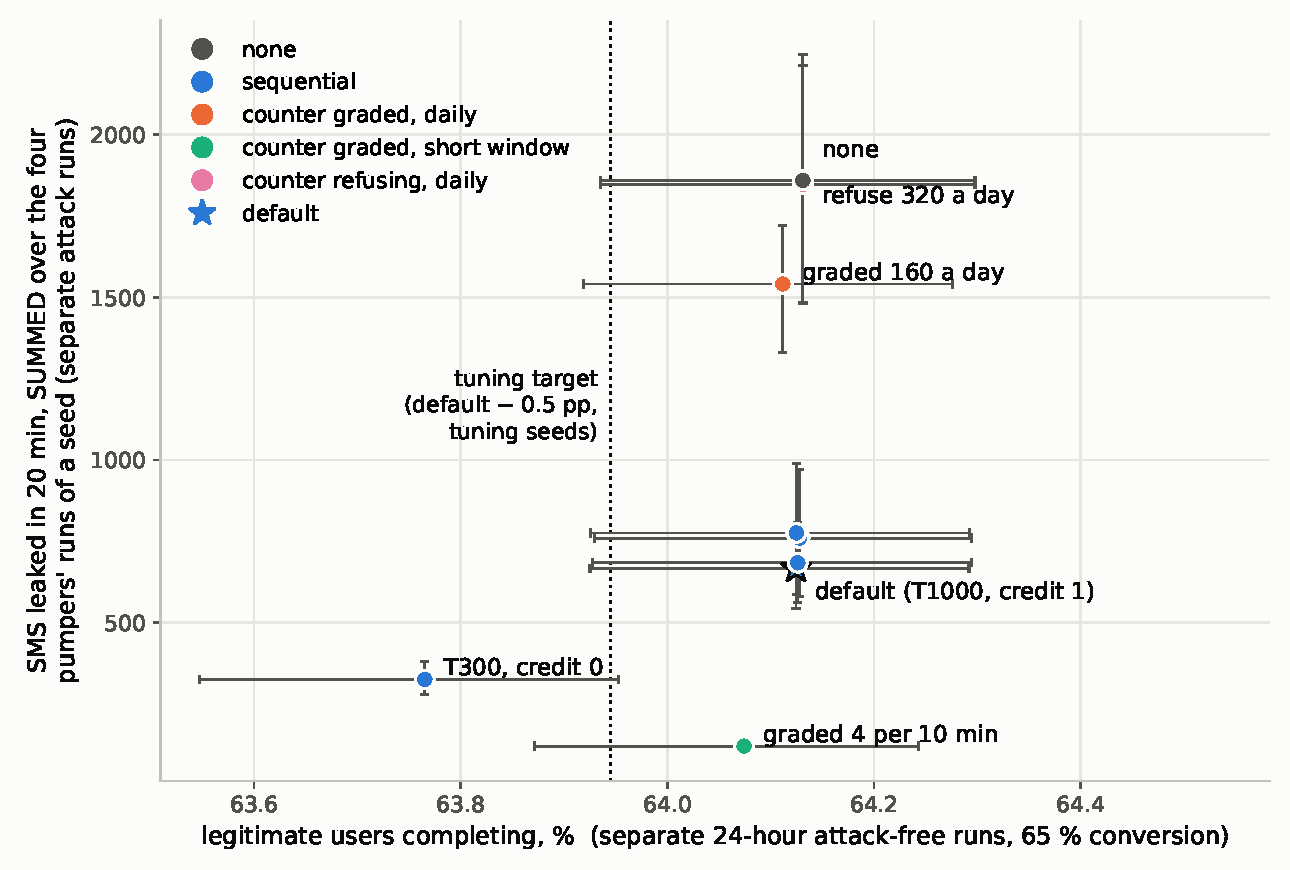
\includegraphics[width=\textwidth]{fig6_matched_a}
\caption{Matched comparison, first protocol, 200 blocks, evaluation seeds 0--9: each setting's completion in 24-hour attack-free runs at 65\% conversion against its 20-minute leakage summed over the four concentrated pumpers' runs of a seed (not one combined attack). Bars: 95\% bootstrap intervals over seeds. Dotted line: the tuning target. Unlabelled points: other sequential settings.}
\label{fig:matched}
\end{figure}

\begin{figure}[!tbp]
\centering
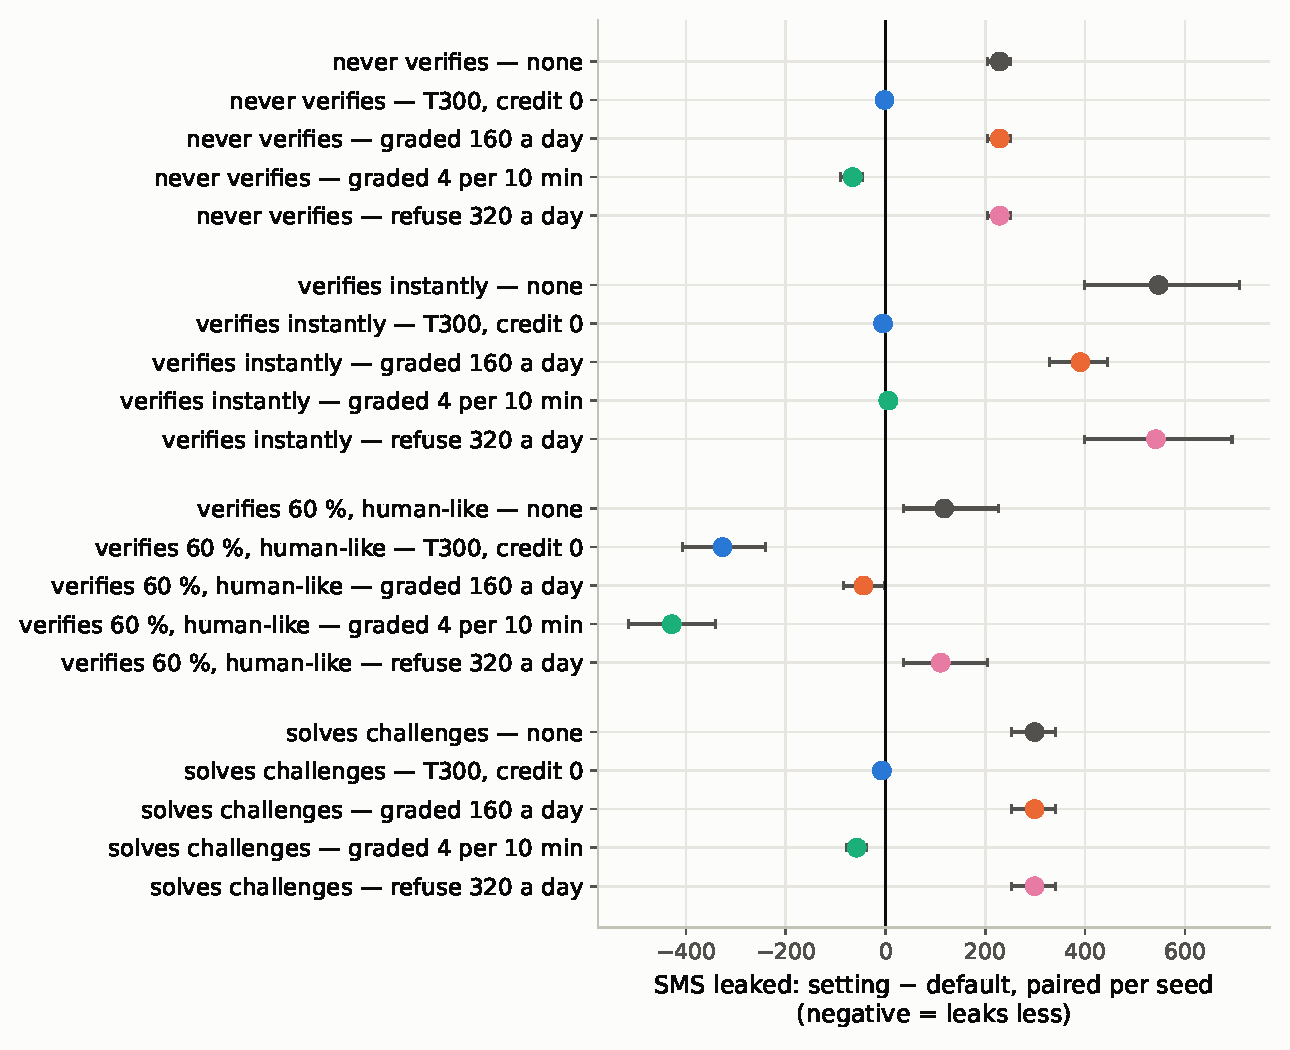
\includegraphics[width=\textwidth]{fig6_matched_b}
\caption{Matched comparison, first protocol, 200 blocks, evaluation seeds 0--9, 20-minute attacks: for each selected setting and each concentrated pumper, the setting's leakage minus the default's, paired per seed (negative: leaks less), with 95\% bootstrap intervals over seeds.}
\label{fig:matchedpaired}
\end{figure}

\begin{table}[t]
\caption{The second protocol's claims for the principal counter (graded, 4 per 10 min) on the held-out family: 12 shifted points, held-out attack rates and pools, three seeds each, a 20-minute pumper on three blocks real users share. A claim holds if true in 90\% of cells; cells share workloads and seeds and are not independent. IV: the instant verifier's cells.}
\label{tab:claims}
\scriptsize
\begin{tabular}{@{}lp{5.0cm}rr>{\raggedright\arraybackslash}p{2.5cm}@{}}
\toprule
Claim & Statement & True / cells & IV & Result \\
\midrule
\tablerows{tables/claims.tex}
\bottomrule
\end{tabular}
\end{table}

\paragraph{Under a second protocol}
Frozen and run on the held-out family (Table~\ref{tab:claims}), the counter leaked 33, 34, 33 and 62 messages against the four carriers, where the default leaked 287, 36, 344 and 287 and no policy 451 to 1\,857, at a benign cost of 0.13 [0.09, 0.17] points, and failed both service-under-attack claims: 13 of the 17 cells that broke K3 lie at the three points with the most legitimate traffic, where users and pumper compete for one quota; K5 failed in 51 cells over 11 of 12 points. The counters selected for sparser traffic cost 4.7 and 5.8 points here even without an attack: the quota must match the traffic.

Table~\ref{tab:attacked} separates three questions. Against the attacked no-policy arm the counter cost all users nothing on average and gained the attacked blocks' users 3 points on average, since without a destination policy the pumper exhausts their blocks and the hourly budget; with the human-like carrier alone it cost them 1.9. Against attack-free operation every evaluated policy still left those users 5 to 9 points worse off (8 with none): none shields a block an attacker shares. Counter and tests together, explored outside the frozen claims, leaked least against the four carriers, but under the poisoner cost all users most of the counters and buckets and leaked more than the tuned sequential setting. A token bucket with a burst of 4 spared the poisoner's users only by letting nearly every message through; with two untuned settings neither limiter dominates, and we rank only the implemented policies. Returning users, simulated as identities with verified history, lost nothing under these policies.

\begin{table}[t]
\caption{Attacked service (E1): 200 blocks, 60-minute attacks, seeds 300--309. Leaked: SMS to the attacker's numbers, in (a) summed over the four carriers' runs of a seed. Harm: net completions lost, in points of all users (about 1\,200 a run) or of the attacked blocks' users (block; about 18 a run), in (a) averaged over the carriers; negative: a gain. Benign: the attack-free cost against no policy. Brackets: 95\% bootstrap intervals over seeds. (a) A pumper on three blocks real users share. (b) A poisoner on all 200 blocks. Per-carrier values: artifact.}
\label{tab:attacked}
\scriptsize
\setlength{\tabcolsep}{1.6pt}
\begin{tabular}{@{}lrrrrrr@{}}
\toprule
\multicolumn{7}{@{}l}{(a) Four concentrated carriers} \\
 & & \multicolumn{2}{c}{Extra harm} & \multicolumn{2}{c}{Degradation} & \\
 & & \multicolumn{2}{c}{vs attacked none} & \multicolumn{2}{c}{vs attack-free} & \\
\cmidrule(lr){3-4}\cmidrule(lr){5-6}
Policy & Leaked & all & block & all & block & Benign \\
\midrule
\tablerows{tables/attacked_a.tex}
\midrule
\multicolumn{7}{@{}l}{(b) Block poisoner} \\
 & & \multicolumn{2}{c}{Extra harm vs attacked none} & & & \\
\cmidrule(lr){3-4}
Policy & Leaked & all & first-time & & & \\
\midrule
\tablerows{tables/attacked_b.tex}
\bottomrule
\end{tabular}
\end{table}

\begin{figure}[!tbp]
\centering
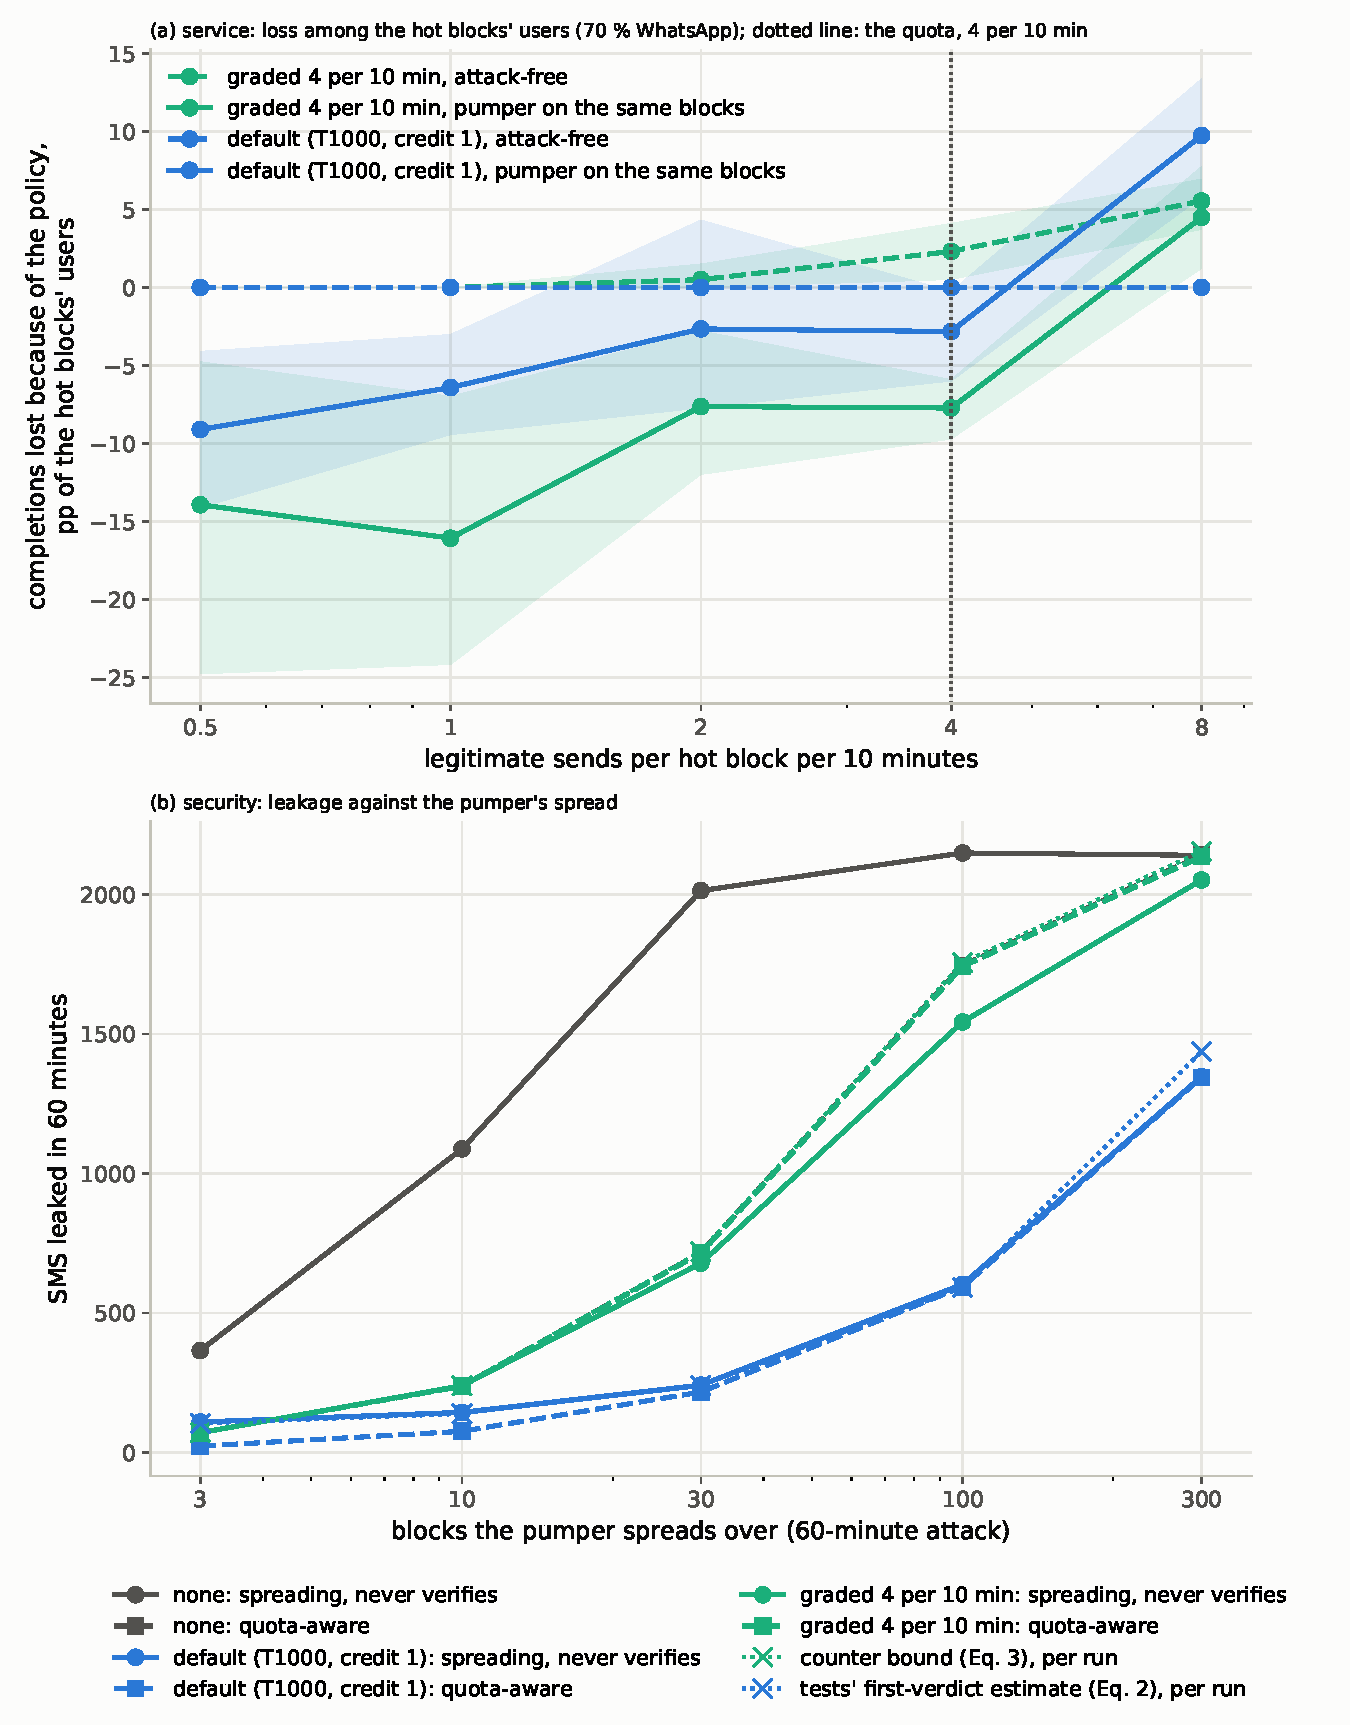
\includegraphics[width=\textwidth,height=0.8\textheight,keepaspectratio]{fig7_counter_boundary}
\caption{The counter's operating boundary (E4), seeds 300--304; lines join sampled settings and do not locate a crossover. (a) Attributable loss in points of the three hot blocks' users (70\% WhatsApp reachability) against their legitimate rate, without and with a never-verifying pumper on those blocks; vertical line: the quota. (b, c) Leakage in 20 and 60 minutes against the blocks a pumper uses, at full rate or paced; dotted: Equations~\eqref{eq:leak} (tests), \eqref{eq:counter} (counter, cold start) and~\eqref{eq:counterwarm} (warm start) for the full-rate pumper, from each run's inputs. Bands and bars: 95\% bootstrap intervals over seeds.}
\label{fig:boundary}
\end{figure}

Attack-free (Figure~\ref{fig:boundary}a), the counter costs a block's users nothing at one send per ten minutes, 2.3 points at four and 5.5 at eight, far below the idealized share beyond the quota (27\% at four), since most challenged users complete or switch to WhatsApp; without WhatsApp eight sends cost 13.2. A 30-minute launch at three times the normal rate costs its blocks' users 16 points. Over 60 minutes (Figure~\ref{fig:boundary}c) the default leaked 110, 144 and 242 messages on 3, 10 and 30 blocks, against 105, 139 and 240 from Equation~\eqref{eq:leak} ($\lambda\tau \approx 90$), and the counter 71, 240 and 679 against its cold-start bound of 72, 240 and 720. No counter run that started cold (44 of 100) exceeded Equation~\eqref{eq:counter}; three warm ones did, by 5 or 6 messages, and none exceeded Equation~\eqref{eq:counterwarm} once 7 messages sent, exempt, to real users' trusted numbers are set aside. With these unfitted inputs Equation~\eqref{eq:cross} ordered the policies' mean leakage in 18 of 18 decisive cells (two ties at $N$), and with the warm-start term in 17, missing where the estimates differ by 0.8 messages (30 blocks, 20 minutes; measured difference 6.6 [$-$27.2, 42.4]); per seed, 76 of 78 decisive comparisons agree. The algebraic crossing lies near five blocks for an hour and 30 for twenty minutes, where the nearest measured differences (three and 30 blocks) do not exclude zero; it is not a measured switching point. A pumper paced to the quota leaks about as much under the counter as with no policy (71 against 72 on three blocks in an hour), and 23 under the tests. Against adaptive attackers (E3) the counter held the threshold-aware carrier, the receipt faker and the concentrated trust builder to 24 to 36 messages (502 to 665 under the default), but not trust builders on random numbers (577, as under the default); over 360 minutes the human-like carrier gained 81 messages an hour under the counter, 753 under the default.

\subsection{RQ5: what destination policies cost legitimate users}
\label{sec:fp}

On one block, 20\,000 Monte Carlo trials per cell give the probability of a verdict within 30 legitimate sends: 0.09\% [0.06, 0.14] at 80\% conversion with 20\% autofill, 1.9\% at 65\% and 19.5\% at 50\%. Over 24 hours the default raises 0.5 verdict events a day on 200 busy blocks at 80\% conversion and 6.5 at 65\%, where they meet 30 of about 28\,800 requests (claim C4 held in 18 of 18 cells).


A poisoner flooding for twenty minutes the twenty blocks legitimate users concentrate on (caps lifted, ten seeds) raises 16 verdict events that meet 98 legitimate requests, 33 never completing; against the observe-only run on the same trace, enforcement costs 12.7 [4.6, 22.9] completions, 3.1\% of users (6.3\% without WhatsApp), and 23.9\% with a 24-hour denylist. One that stops after ten minutes leaves verdicts that meet 406.5 requests afterwards, an attributable loss of 46.2 [16.9, 79.8] (48.2 over the whole run). Grading limits the harm; it caps it neither at a challenge nor at the attack's duration.

\subsection{Adaptive attackers, economics and overhead}
\label{sec:adaptive}

These scripted adaptations' leakages are not bounds. Against v2 with caps lifted, a datacenter attacker buying every challenge solution leaks 55; a threshold-aware carrier and a receipt faker leak 570 each, drawing no verdict.

If pumpers earn a share of the 0.1422 USD retail price and pay an event-level bill, they break even at a share of 0.043 under v1 and 0.054 to 0.271 under v2 (the instant verifier 1.310); over 360 minutes under the counter the human-like carrier needs 1.048. These are break-even shares for scripted attackers under assumed prices, not bounds or criminal profit.

On a real Redis (four vCPUs, four workers), a send costs 13.8\,ms (median) and 21.1\,ms (99th percentile). With the 400\,ms floor and 50\,ms vendor calls, throughput reaches 133 requests per second at concurrency 128. With fast vendors no pair of five outcome classes was distinguished (smallest Kolmogorov--Smirnov $p = 0.051$; best single-threshold accuracy 53\%). Under an adversarial mixture with heavy-tailed vendors at concurrency 128, 81\% of sends overran the floor in server time, and a threshold on client response times separated that run's 2\,497 sends from its 22 refusals with 88\% balanced accuracy (resubstitution); on three new runs, thresholds fitted on one run scored 95 to 99.9\% on the other two: a separation on that machine, not a deployment accuracy.

% ---------------------------------------------------------------------------
\section{Discussion}
\label{sec:discussion}

\paragraph{Lessons}
In the scripted workloads, carriers that verify with human-like delay, fake receipts or know the thresholds defeated our outcome tests but not a short-window counter. Within a verdict's hour the counter's allowance, unlike the tests', grows with the windows an attack spans; over longer campaigns verdicts expire and the tests leak again. Equation~\eqref{eq:cross} summarizes this for pumpers that solve no challenge and hold no exemption. Its inputs are in an operator's logs and timeouts; the cost of an excess send, competition under attack and exemption abuse come only from the simulation. Counter and tests together, with a quota set from each block's traffic, is a hypothesis for real traffic, not a recommendation.

\paragraph{Limitations}
Everything is simulated and the calibration is assumed. Both protocols were written by the author for the author's generator, the second knowing which counters had won. Some results follow from the generator (a perfect premium list, a datacenter attacker that declines challenges, returning users who always present verified history), and selection used an unweighted sum of four scripted pumpers' leakage and a mean service target. Close rankings rest on ten or fewer seeds, and costs that round to zero are not shown equivalent. Per-client quotas within a block, carrier spend ceilings, bounded exemptions, tuned token buckets and other sequential statistics lie outside the evaluated policies. Vendor adapters are untested live, and the timing result holds only for the observer model tested. Destination policies challenge people for what strangers sharing their block did, and deployment under the GDPR or Saudi Arabia's PDPL needs a lawful basis and a route for refused users. Replaying real traffic is the experiment this paper most needs.

% ---------------------------------------------------------------------------
\section{Conclusion}
\label{sec:conclusion}

In this simulation the design contains attacks that carry a signature at little cost to simulated users, and rations, rather than separates, a residential attacker that looks like a person. Counting sends on the destination leaked less in aggregate than our outcome tests against concentrated pumpers, though not reliably against an instantly verifying carrier; a frozen counter failed its service claims when the attacker shares blocks with real users, and lost its advantage against wide, paced and trust-building pumpers. Within an hour, unfitted estimates order the two policies in every decisive boundary cell, as an algebraic crossing, not a measured switching point.

\section*{CRediT authorship contribution statement}
\textbf{Naveed Ahmed:} Conceptualization, Methodology, Software, Validation, Investigation, Writing -- original draft, Writing -- review \& editing.

\section*{Declaration of competing interest}
The author declares no known competing financial interests or personal relationships that could have appeared to influence this work.

\section*{Declaration of generative AI and AI-assisted technologies in the writing process}
The author used Claude (Anthropic) for code, evaluation, drafting and editing, checked numbers against the recorded results and claims against the code, and takes full responsibility for the content.

\section*{Data availability}
{\raggedright No human or real traffic data was used. Code, protocols (\texttt{config/}), every run's configuration and outcome (\texttt{results/}), the comparison with the 2.8.0 results (\texttt{store\_change\_report.md}) and the sources of headline numbers (\texttt{headline\_numbers.md}) are at \url{https://github.com/nahmedpsu/OTP-DDOS}, release 2.9.0 (tag v2.9.0), which produced the results; the 2.8.0 results are in \texttt{results/\allowbreak historical\_2.8}. These files are the supplementary material.\par}

\bibliographystyle{elsarticle-num}
\bibliography{refs}

\end{document}
